\documentclass[11pt]{article}
\usepackage[utf8]{inputenc}
\usepackage[T1]{fontenc}
\usepackage{graphicx}
\usepackage[export]{adjustbox}
\graphicspath{ {./images/} }
\usepackage{hyperref}
\hypersetup{colorlinks=true, linkcolor=blue, filecolor=magenta, urlcolor=cyan,}
\urlstyle{same}
\usepackage{amsmath}
\usepackage{amsfonts}
\usepackage{amssymb}
\usepackage[version=4]{mhchem}
\usepackage{stmaryrd}

\begin{document}
Overview of Funds of Hedge Funds

The preceding five sessions have described the universe of hedge funds and its constituent categories of macro and managed futures, event-driven, relative value, and equity strategies. Few investors allocate their entire hedge fund investment to a single hedge fund manager or even a single hedge fund strategy. Investors realize that each manager and each strategy has its own specific risks and cyclicality of returns and that diversification across managers and strategies can reduce the risks of hedge fund investing.

The hedge fund industry includes funds of funds (FoFs) as well as single-manager funds. Funds of funds are hedge funds with an underlying portfolio of other hedge funds. The primary advantages of a fund of funds are diversification, professional manager selection, and portfolio management processes. The primary disadvantage of a fund of funds is a second layer of fees imposed by the fund of funds manager.

Investors may also want to consider multistrategy funds, which manage multiple strategies within a single entity. Multistrategy funds offer strategy diversification without the additional layer of fees, but there are also trade-offs involved when selecting these funds.

A fund of hedge funds is a diversified fund run by a single hedge fund manager, in which assets are allocated among other hedge funds. This structure creates two layers of fees: the fees of the fund of funds structure, and the fees of the underlying hedge fund investments. A key goal of investing in a fund of funds is to improve portfolio diversification, as a fund of funds quickly diversifies both the risks of concentrated hedge fund styles and the idiosyncratic risks of investing with single hedge fund managers.

\section*{Benefits and Costs of Diversification}
The benefits of holding a diversified portfolio of assets result from correlations among asset returns being less than 1, meaning that returns are not perfectly positively correlated. The next exhibit shows that there have been varying correlations across hedge fund strategies, ranging from 0.247 between macro and relative value to 0.915 between event-driven and equity hedge. Because each hedge fund strategy has its own risks and varying correlations to other hedge fund strategies, diversifying across hedge fund strategies reduces the risk of a hedge fund portfolio. As shown in the exhibit below, with a correlation of 0.855 to the MSCI World Index and 0.029 to the Bloomberg Barclays US Aggregate Bond Index, the HFRI Fund Weighted Composite Index also brings diversification and risk reduction to a portfolio of traditional stock and bond investments.

Correlation of Returns across Investment Strategies, January 2000 to December 2020

\begin{center}
\begin{tabular}{|c|c|c|c|c|c|c|c|c|}
\hline
\begin{tabular}{l}
(Jan. 2000-Dec. \\
2020) \\
\end{tabular} & \begin{tabular}{l}
MSCI \\
World \\
Index \\
\end{tabular} & \begin{tabular}{l}
Bloomberg Barclays \\
US Aggregate Bond \\
Index \\
\end{tabular} & \begin{tabular}{c}
HFRI Fund \\
Weighted \\
Composite Index \\
\end{tabular} & \begin{tabular}{l}
HFRI Fund of \\
Funds Composite \\
Index \\
\end{tabular} & \begin{tabular}{l}
HFRI Macro \\
(Total) \\
Index \\
\end{tabular} & \begin{tabular}{l}
HFRI Event- \\
Driven (Total) \\
Index \\
\end{tabular} & \begin{tabular}{l}
HFRI Relative \\
Value (Total) \\
Index \\
\end{tabular} & \begin{tabular}{c}
HFRI Equity \\
Hedge (Total) \\
Index \\
\end{tabular} \\
\hline
MSCI World Index & 1.000 &  &  &  &  &  &  &  \\
\hline
\begin{tabular}{l}
Bloomberg Barclays \\
US Aggregate Total R \\
\end{tabular} & 0.027 & 1.000 &  &  &  &  &  &  \\
\hline
\begin{tabular}{l}
HFRI Fund Weighted \\
Composite Index \\
\end{tabular} & 0.855 & 0.029 & 1.000 &  &  &  &  &  \\
\hline
\begin{tabular}{l}
HFRI Fund of Funds \\
Composite Index \\
\end{tabular} & 0.748 & 0.045 & 0.951 & 1.000 &  &  &  &  \\
\hline
\begin{tabular}{l}
HFRI Macro (Total) \\
Index \\
\end{tabular} & 0.299 & 0.233 & 0.533 & 0.556 & 1.000 &  &  &  \\
\hline
\begin{tabular}{l}
HFRI Event-Driven \\
(Total) Index \\
\end{tabular} & 0.803 & -0.024 & 0.935 & 0.897 & 0.364 & 1.000 &  &  \\
\hline
\begin{tabular}{l}
HFRI Relative Value \\
(Total) Index \\
\end{tabular} & 0.680 & 0.114 & 0.818 & 0.835 & 0.247 & 0.869 & 1.000 &  \\
\hline
\begin{tabular}{l}
HFRI Equity Hedge \\
(Total) Index \\
\end{tabular} & 0.870 & -0.013 & 0.984 & 0.928 & 0.450 & 0.915 & 0.790 & 1.000 \\
\hline
\end{tabular}
\end{center}

The next exhibit, Estimated Strategy Composition by Assets Under Management, 4Q 2021 shows how investors have chosen to allocate their total investment in hedge funds to various strategy types. The largest allocation to single-strategy managers has been to equity hedge, and relative value managers and event-driven funds have earned larger allocations than have macro managers. At the end of 2021, Hedge Fund Research (HFR) estimated that the industry was composed of 8,185 single hedge funds and 1,069 funds of funds. Whereas the number of single-manager hedge funds continues to grow, there has been consolidation in the funds of funds sector, as there were 2,462 funds of funds at the end of 2007 .

\begin{center}
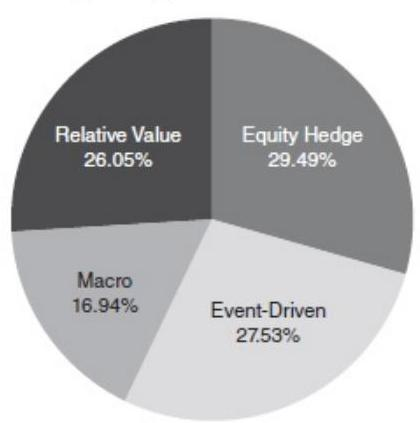
\includegraphics[max width=\textwidth]{2024_04_09_a22e8e8765db4383bf63g-3}
\end{center}

Estimated Strategy Composition by Assets Under Management, 4Q 2021

Source: HFR Industry Reports, HFR, Inc. (C) 2021, \href{http://www.hedgefundresearch.com}{http://www.hedgefundresearch.com}.

\section*{Four Functions of Fund of Funds Management}
Delegated management using a fund of funds (FoF) approach provides investors with professional management to perform the following four important functions:

\begin{enumerate}
  \item Strategy and manager selection: The FoF manager is responsible for selecting the strategies and the managers who will implement those strategies. FoF managers may have access to closed managers as well as insights regarding strategies that are likely to perform better going forward. Many of the largest institutional investors and their investment consultants have teams dedicated to finding, vetting, and investing directly in hedge funds.

  \item Portfolio construction: Once the strategies and managers have been selected, the FoF manager has to decide on how much to allocate to each strategy and manager. The allocation will depend on the risk and return characteristics of the individual managers and the expected correlations between funds, as well as other fund features, such as the lockup period, the liquidity of the positions, the size of the fund, and the length of each manager's track record.

  \item Risk management and monitoring: The FoF manager will monitor each hedge fund to ensure that its ongoing performance profile is consistent with the fund's overall objectives. Some FoFs employ sophisticated risk-management processes to monitor the underlying hedge funds' positions. Other FoFs may employ multifactor sensitivity analysis to gauge the risk exposure to various market factors and to analyze the funds' potential tail risk.

  \item Due diligence: For hedge fund investing, due diligence is the process of monitoring and reviewing the management and operations of a hedge fund manager. This is perhaps one of the more important functions and value-added features of an FoF manager to consider when deciding between a direct and a delegated hedge fund investment program. Unfortunately, some of the large FoFs have been marred by blowups and fraud scandals, which have caused some institutional investors to become wary about the value of an FoF's due diligence process. There is, however, some academic evidence justifying the payment of an additional layer of fees in return for operational due diligence. Operational due diligence is the process of evaluating the policies, procedures, and internal controls of an asset management organization. Brown, Fraser, and Liang ${ }^{1}$ Stephen J. Brown, Thomas L. Fraser, and Bing Liang (January 21, 2008), Hedge Fund Due Diligence: A Source of Alpha in a Hedge Fund Portfolio Strategy, SSRN: \href{https://papers.ssrn.com/sol3/papers.cfm?abstract}{https://papers.ssrn.com/sol3/papers.cfm?abstract} id=1016904. estimate that net of fees, the largest FoFs tend to outperform the smallest FoFs. Larger FoFs may outperform because their scale allows them to invest greater resources in due diligence and risk management processes.

\end{enumerate}

\section*{Eleven Benefits to Investing in Funds of Funds}
In addition to accessing professional management for the four functions just discussed, there are a number of other benefits to investing in funds of funds. These potential benefits include the following 11 advantages:

\begin{enumerate}
  \item Diversification: Prudent investing dictates that portfolios be well diversified. Some investors lack the necessary asset size and expertise to invest directly in hedge funds to reach an appropriate level of diversification and risk reduction. By contrast, through a single FoF investment, investors can access a welldiversified portfolio in terms of managers or strategies. However, the diversification level of an FoF portfolio is not necessarily a straightforward function of the number of underlying funds or strategies analogous to stock investing. This is because hedge funds are not single securities; rather, they are previously diversified portfolios of securities.

  \item Accessibility: The median minimum investment for a single hedge fund is $\$ 500,000$, which makes diversification into numerous funds unaffordable for most individual investors. By comparison, minimum investment levels for FoFs are relatively low. This allows more individual investors and small institutions to gain diversified access to hedge funds even though their capital base is comparatively small.

  \item Economies of scale: Investors essentially share costs, such as those associated with the manager selection, reporting, analysis, and due diligence processes, with their FoF co-investors, thereby reducing their individual costs.

  \item Information advantage: As professional asset allocators, FoF managers have the ability to access, collect, and interpret data gleaned from various channels, such as data providers, prime brokers, and industry contacts. This gives them an informational advantage over nonprofessional investors.

  \item Liquidity: Investments in hedge funds are relatively illiquid, due to lockups, potential redemption gates, notice periods, and limited redemption dates. By comparison, the liquidity terms offered by FoFs are typically more flexible. Most FoFs offer quarterly or monthly liquidity in normal market conditions. Some FoFs even offer daily liquidity, either through a listing on an exchange or via an over-the-counter secondary market that matches demand and supply.

  \item Access to certain managers: Access to the best talent and ideas in the hedge fund community is a scarce resource. The most desirable hedge funds may be closed to new investments. Many investors do not have the necessary networks and protocol for obtaining investment capacity in these funds when it becomes available. Investing in an existing FoF that is already allocated to these desirable hedge funds is the fastest way to immediately participate in their performance.

  \item Negotiated fees: Thanks to the power of their collective assets, some FoFs have successfully negotiated access to certain managers at reduced fees. This is normally beyond the capabilities of most individual investors.

  \item Regulation: In order to facilitate their distribution to a wider audience, some FoFs choose to register in regulatory jurisdictions that offer better investor protection than their underlying investments, even though the cost and administrative and operational burdens may be higher. The improved investor protections can often be reassuring for first-time investors and can ensure that they will receive sufficient transparency, oversight, and quarterly reports.

  \item Currency hedging: Although the currency of choice in the hedge fund world is the US dollar, some FoFs offer share classes denominated in various currencies with the currency risk hedged. Whereas institutional investors often wish to manage their own currency risks, many small or private investors prefer to be\\
shielded from currency fluctuations and thus delegate the hedging aspects to professional managers.

  \item Leverage: Some FoFs provide leverage to their investors. They borrow money in addition to the capital provided by their investors and invest it in a portfolio of hedge funds. This allows them to produce higher returns than would be produced with an unlevered FoF, as long as the leverage and interest costs incurred are surpassed by the unlevered returns of the underlying hedge fund portfolio.

  \item Educational role: Many first-time hedge fund investors look at FoFs not simply as an investment vehicle but as a way of learning about hedge fund strategies and hedge fund managers. Larger investors may switch to direct investments in hedge funds after gaining a few years of experience.

\end{enumerate}

\section*{Six Disadvantages to Investing in Funds of Funds}
Conversely, there are disadvantages to investing in funds of funds. These include the following six potential disadvantages:

\begin{enumerate}
  \item Double layer of fees: FoF managers effectively pass on to their investors all fees charged by the underlying hedge funds in their portfolios, while also charging an extra set of fees for their own work, as well as for an additional layer of service providers. Many FoFs charge a $1 \%$ management fee and a $10 \%$ performance fee on top of an underlying hedge fund management fee of sometimes $2 \%$ and an incentive fee of $20 \%$ for the hedge funds. Due to economies of scale, institutional investors making large allocations have recently been paying much lower fees than the $1 \%$ and $10 \%$. Fees have been falling in recent years, due to both disappointing hedge fund performance and the increased buying power of large investors. As of 2021, the median hedge fund charges a management fee of $1.5 \%$ and an incentive fee of $17.5 \%$, with just $30 \%$ charging $2 \%$ and $20 \%$. As far as funds of funds go, the median is now a $0.8 \%$ management fee and an incentive fee of $9 \%$. Funds of funds are increasingly available, with incentive fees between $0 \%$ and $5 \%$.

  \item Performance fees not netted: In an FoF, the investor must pay performance fees for each of the underlying hedge funds that are profitable, regardless of the performance of the overall portfolio. Thus, if half the managers are down $10 \%$ and the other half are up $10 \%$ on a gross basis, the investor will have to pay a performance fee to the positive performers despite no positive returns at the aggregate level. The fees are the same for portfolios of funds using direct investing. However, the fees are generally lower using a multistrategy fund, discussed later, because performance fees are charged on a netted or aggregate basis.

  \item Taxation: Because of their offshore registration, many hedge funds and FoFs may be tax inefficient for certain investors in certain countries. As an illustration, in Germany, most FoFs invest in hedge funds that fail to meet the extensive notification and disclosure duties requested by the German authorities. As a result, their gains are subjected to heavy taxation penalties, which ultimately affect the investor.

  \item Lack of transparency: Some FoF managers do not disclose the content of their portfolio or their asset allocation. They contend that it represents the valuable skills that they bring to the table, and they are reluctant to reveal their full strategy. In such cases, it becomes relatively difficult for their investors to understand what is really happening in terms of risk and returns beyond the information that can be ascertained from the stream of net asset values (NAVs).

  \item Exposure to other investors' cash flows: FoFs commingle the assets of a number of investors. As a result, investors are affected jointly by inflows and outflows, since co-investors in the same fund may trigger cash increases or decreases or undesirable leveraging to finance redemptions. Furthermore, to satisfy investors' requests for redemption, the FoF manager will typically sell the most liquid funds first, leading to a potential change in the FoF's style. Custom portfolios for a single investor (managed accounts) are not exposed to this type of problem.

  \item Lack of control: In an FoF, investors give up control over how the assets are managed. Moreover, they lose the direct relationship with the hedge funds in which the FoF invests. Direct investment in hedge funds allows investors to create allocations that fit their overall portfolios, but investors in FoFs can't control this style allocation. For example, the pension fund of a bank may not wish to have exposure to distressed credit instruments because of the business risk of the pension fund's sponsor.

\end{enumerate}

\section*{Three Major Ways for FoF Managers to Add Value}
One of the most important debates with respect to FoFs concerns whether they deserve their second layer of fees. For example, do funds of funds add value relative to a direct investing approach that randomly selects a portfolio of, say, 20 to 40 hedge funds? In practice, there are essentially three major ways for FoF managers to add value from portfolio selection and asset allocation:

\begin{enumerate}
  \item Through strategic allocations to various hedge fund styles: Running an FoF is not just simply a matter of assembling a large collection of good managers. Having such a collection can still result in a concentration of risks, with somewhat illusory diversification if there is a high level of correlation in the trades or underlying exposures of these managers. The first choice that an FoF manager must make when organizing a portfolio is the long-term strategic asset allocation. The strategic allocation sets the long-term weights across strategies, such as static weights of $20 \%$ on macro strategies and $30 \%$ on equity strategies.
\end{enumerate}

This normally implies analyzing the long-term risk and return profiles of the different strategies, as well as examining the correlation of their observed and expected returns. The goal is then to determine an initial portfolio allocation consistent with the fund's long-term objectives and constraints. This task determines the long-run beta of the fund with respect to various sources of risks. Superior strategic asset allocations would be an important way for a fund of funds manager to add value.

\begin{enumerate}
  \setcounter{enumi}{1}
  \item Through tactical allocations across hedge fund styles: Tactical asset allocation refers to active strategies that seek to enhance short-term portfolio performance by opportunistically shifting the asset allocation in response to the changing environment. Many FoFs argue that they implement a top-down, tactical allocation process. In theory, this involves making three key style-weighting decisions periodically: (1) what to do (i.e., overweighting or underweighting a particular investment style); (2) when to do it (i.e., implementing the changes based on levels of certain indicators or factors); and (3) how much to do (i.e., deciding whether the overweight should be, for example, $1 \%$ or $3 \%$ ).
\end{enumerate}

In practice, however, an FoF's tactical allocations are limited due to the underlying hedge funds' liquidity constraints unless the fund of funds invests in the most liquid areas of alternative investments or uses managed accounts. However, new investment flows received by the FoF can be used to reallocate to the most attractive tactical opportunities. Thus, tactical allocation may be a way for fund of funds managers to add value by determining how much the FoF adjusts its asset allocations in response to changes in the market environment.

\begin{enumerate}
  \setcounter{enumi}{2}
  \item Through selection of individual managers: FoF managers can add value within a strategy through the decision of how much money to invest with each manager. Although this manager selection activity seems very similar to a traditional stock selection activity, the reality is that FoF managers need to consider the liquidity of the funds. Managers have to make a trade-off between their ability to add value through dynamic manager allocations in highly liquid funds and the potential contribution of less liquid funds (those with lockups, etc.). Managerial selection can be a major source of added value for an FoF manager.
\end{enumerate}

The first issue to consider when constructing a portfolio of hedge funds is how many funds are needed to achieve appropriate diversification. That is, how many funds are required to reduce manager- and style-specific risks while maintaining manager weights large enough for superior manager selection to have a positive impact on the portfolio? We discuss two methods of estimating the relationship between number of funds and level of diversification: empirical and theoretical.

Using the empirical approach, Fothergill and Coke suggest that a broadly diversified portfolio of between 15 and 20 hedge funds can reduce portfolio volatility to the level of fixed-income investments. ${ }^{2}$ Martin Fothergill and Carolyn Coke (Fall 2001), Funds of Hedge Funds: An Introduction to Multi-Manager Funds, Journal of Alternative Investments 4 (no. 2): 7-16. Amo, Harasty, and Hillion measure the impact of each additional hedge fund investment on the standard deviation of terminal wealth. ${ }^{3}$ Anne-Valere Amo, Helene Harasty, and Pierre Hillion (Fall 2007), Diversification Benefits of Funds of Hedge Funds: Identifying the Optimal Number of Hedge Funds, Journal of Alternative Investments 10 (no. 2): 10-21. At a one-year time horizon, a portfolio of eight hedge funds has half of the standard deviation of a single hedge fund, and investing in as few as five funds cuts the risk by more than half at a time horizon of 5 or 10 years. The marginal risk reduction benefit of adding more than 15 to 20 hedge funds is minimal. Gregoriou states that portfolios of more than 40 hedge funds dilute manager skill and approach the risk and return of a hedge fund index. ${ }^{4}$ Greg Gregoriou (Winter 2004), Are Managers of Funds of Hedge Funds Good Market Timers? Journal of Wealth Management 7 (no. 3): 61-76.

The problem with the empirical approach to estimating the benefits to diversification is differentiating between systematic and diversifiable risks and the assumption that future returns will offer the same levels of diversification indicated by analysis of past returns. A theoretical approach is to model the returns of a portfolio as depending on the weights, variances, and covariances of the returns of the constituent assets. Equation 2 from the lesson Interpreting Standard Deviation and Variance, replicated here, reflects Markowitz's pioneering expression for the variance of a portfolio when the assets are uncorrelated:

$$
V\left(R_{p}\right)=\sum_{i=1}^{n} w_{i}^{2} \operatorname{Var}\left[R_{i}\right]
$$

when $\rho=0$ between all $n$ individual assets.

To derive a simple rule, this equation is used while assuming that all assets in the portfolio are equally weighted, all assets have no systematic risk, and all assets have equal variances, $\sigma^{2}$. In this case, the variance of the portfolio is $\sigma^{2} / n$. Given these assumptions, the standard deviation of the rate of return on the portfolio is directly related to the number of funds, as indicated in Equation 1:


\begin{equation*}
\sigma_{p}=\sigma_{f} / \sqrt{n} \tag{1}
\end{equation*}


where $\sigma_{p}$ is the standard deviation of the portfolio's return, $\sigma_{f}$ is the standard deviation of every constituent fund, and $n$ is the number of assets in the portfolio.

Equation 1 provides a simple approximation of risk reduction based on the number of funds. If there are four funds, Equation 1 approximates that the standard deviation of the portfolio will be half the standard deviation of a single fund. Portfolios with 16 and 100 funds will have $75 \%$ and $90 \%$ less standard deviation than a single fund. Equation 1 assumes zero correlation between fund returns, which overstates the benefits to diversification. However, these results may provide reasonable indications of the potential reduction in the idiosyncratic risks.

\section*{Identifying Funds for an Institutional Portfolio or Fund of Funds}
The second issue to consider is that of manager selection and due diligence, described in the Level II curriculum of CAIA. Out of thousands of single-manager hedge funds, how does the portfolio manager attempt to select the best mix of perhaps 20 managers? Many hedge fund investors have one or more simple rules that immediately reduce the number of hedge funds under consideration. For example, a size rule requiring minimum assets under management (AUM) of $\$ 200$ million immediately reduces the number of funds under consideration to less than 1,400 .

The manager funnel, as shown in the next exhibit, shows the steps taken to select a small number of managers from the vast sea of candidates. Quantitative screens, such as a minimum length of track record, minimum returns, or maximum risk when compared to funds in the same style, can also quickly reduce the number of hedge funds under investment consideration. Other criteria may include manager capacity and the ability of the fund of funds manager to build a long-term relationship with the hedge fund manager. The next step, due diligence, is the most expensive and most challenging, beginning with locating and meeting each hedge fund manager. Although locating managers can be accomplished through database searches, many fund of funds managers have an edge through proprietary knowledge of managers who do not report their returns to databases. Large investors are also frequently contacted by managers who wish to present their funds for investment consideration.

\begin{center}
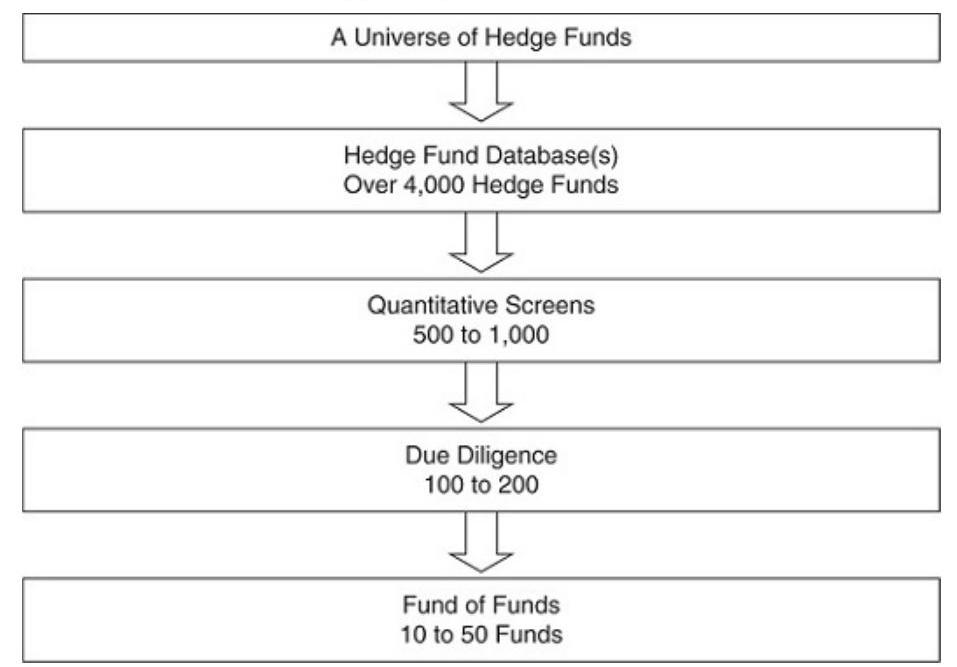
\includegraphics[max width=\textwidth]{2024_04_09_a22e8e8765db4383bf63g-6}
\end{center}

\section*{Hedge Fund Selection}
Suppose that after the quantitative screens and the first manager interview, the portfolio manager has selected an initial 100 to 200 funds for further consideration. Perhaps there are 10 to 20 funds in each investment style. Once the portfolio manager is initially satisfied with this group of candidates, the in-depth due diligence process begins. After reviewing a completed due diligence questionnaire, the investor visits the hedge fund manager's office. The on-site visit gives the investor an opportunity to interview a broad number of staff members from the hedge fund to determine the manager's level of skill and ability to manage market risks and minimize operational risks. The prospective investor should also conduct reference checks, contact service providers, and verify systems and trading programs.


\end{document}